\begin{figure}[H]
  \centering
  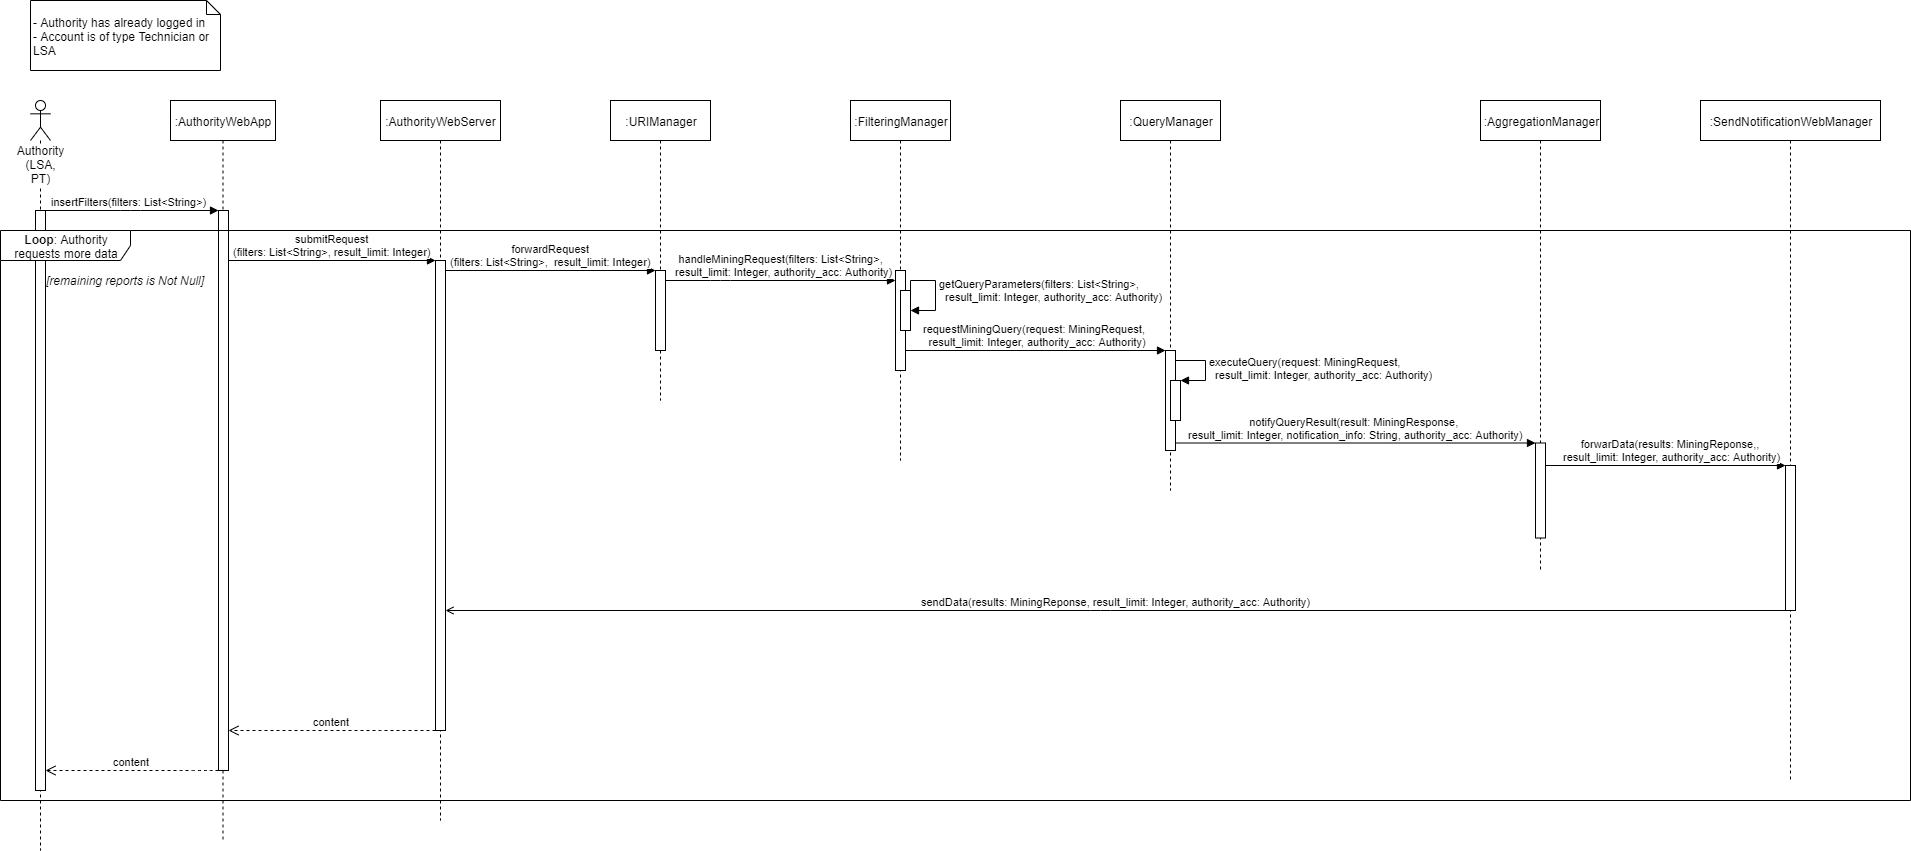
\includegraphics[width=1\textwidth]{Images/UML_diagrams/Sequence_Diagrams/Mine_information_sd.png}
  \caption{Mine information sequence diagram}
  \label{fig:mine_info_sd}
\end{figure}
This sequence diagram shows the workflow of a generic mining request performed by an officer. On the web application the authority can select a set of filters that will define the mining request. Upon submit, the request goes to the AuthorityWebServer component that will have to ask to the Application server the data in order to create the web page to be delivered to the client-side. The AuthorityWebServer will then forward the request, containing the list of filters, to the URIManager which in turn sends the request to the FilteringManager. The latter then collects the parameters necessary for the query, considering the filters inserted by the authority, and successively requests to the QueryManager the execution of a select query based on those parameters. As soon as the execution is complete, the QueryManager will send the mining response to the AggregationManager that will pack it into a standard format. After that it will send the data to the SendNotificationWebManager that will forward it back to the authority. It is important to note that since a mining request can result in a lot of data, a parameter called result\_limit is sent along with the request in order to identify the number of results that we want to return. For example, if an authority makes a request that results in 100 rows, by default the web app will populate the result page with the first 50 entries (default value can be modified in the web app configuration) but if the authority wants to see more data, than he can click on the appropriate button that will perform the same request but with the result\_limit parameter set to 2, to indicate that he wants another 50 data to be displayed. 
% TODO: Check last part
